\documentclass[t]{beamer}
\usetheme{Copenhagen}
\setbeamertemplate{headline}{} % remove toc from headers
\beamertemplatenavigationsymbolsempty

\usepackage{amsmath, array, tikz, bm, pgfplots, tcolorbox, graphicx, venndiagram, color, colortbl, xfrac}
\pgfplotsset{compat = 1.16}
\usepgfplotslibrary{statistics}
\usetikzlibrary{calc}

\title{Sampling Distributions}
\author{}
\date{}

\AtBeginSection[]
{
  \begin{frame}
    \frametitle{Objectives}
    \tableofcontents[currentsection]
  \end{frame}
}

\begin{document}

\pgfmathdeclarefunction{gauss}{2}{%
  \pgfmathparse{1/(#2*sqrt(2*pi))*exp(-((x-#1)^2)/(2*#2^2))}%
}

\begin{frame} 
\maketitle
\end{frame}

\section{Obtain a sampling distribution of sample means}

\begin{frame}{Sampling Distributions}
In statistics, we take samples in order to gather information regarding a population. \newline\\	\pause

For instance, let's say we have the following population prices of laptops: \$1000, \$1200, \$1600, and \$2000.	\newline\\	\pause

We can take a simple random sample of, say 2 computers, and create a frequency distribution of each sample.	\newline\\	\pause

\emph{Note}: We will sample with replacement. Differences in sampling with and without replacement become negligible as sample sizes increase.
\end{frame}

\begin{frame}{Example 1}
Obtain a sampling distribution, taking 2 at a time, of the laptop prices \$1000, \$1200, \$1600, and \$2000. Then find the mean of each sample.	\newline\\	\pause
\begin{minipage}{0.4\textwidth}
\begin{tabular}{c|c}
Sample & Sample Mean \\ \hline
1000, 1000 & 1000 \\
1000, 1200 & 1100 \\
1000, 1600 & 1300 \\
1000, 2000 & 1500 \\
1200, 1000 & 1100 \\
1200, 1200 & 1200 \\
1200, 1600 & 1400 \\
1200, 2000 & 1600 \\
\end{tabular}
\end{minipage}
\hspace{0.5cm}
\begin{minipage}{0.4\textwidth}
\begin{tabular}{c|c}
Sample & Sample Mean \\ \hline
1600, 1000 & 1300 \\
1600, 1200 & 1400 \\
1600, 1600 & 1600 \\
1600, 2000 & 1800 \\
2000, 1000 & 1500 \\
2000, 1200 & 1600 \\
2000, 1600 & 1800 \\
2000, 2000 & 2000 \\
\end{tabular}
\end{minipage}
\end{frame}

\begin{frame}{Example 2}
Create a histogram of the sample means from Example 1.	\newline\\	\pause
\begin{center}
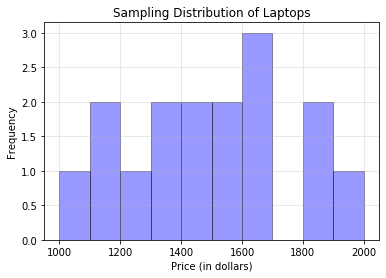
\includegraphics[scale=0.6]{../Images/sampling_hist_01.png}
\end{center}
\end{frame}

\begin{frame}{Example 3}
Determine the mean and standard deviation of the sample means.	\newline\\	\pause

$\text{Mean} = \$1450$ \newline\\	\pause

$\text{Std. Dev} \approx \$271.57$
\end{frame}

\section{Determine the mean and standard error of a sampling distribution}

\begin{frame}{Larger Population and Sample Sizes}
What happens if we have a much larger population and take a larger sample size, such as 100?	\newline\\	\pause

Notice that the mean of the sample means targets the population mean. 	\pause

\[\mu \approx \mu_{\overline{x}}\]		\pause

Also, the standard deviation is around 1/10 the population standard deviation. 	\pause

\[\sigma \approx \frac{\sigma_{\overline{x}}}{\sqrt{n}}\]

where $\frac{\sigma}{\sqrt{n}}$ is called the {\color{blue}\textbf{standard error of the mean}}.
\end{frame}

\begin{frame}{Example 4}
IQ scores are normally distributed with a mean of 100 and standard deviation of 16. A sample of 200 participants had their IQs measured.	\pause
\begin{center}
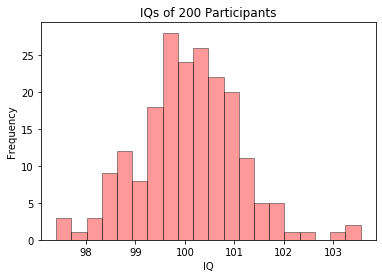
\includegraphics[scale=0.45]{../Images/sample_means_IQ.png}
\end{center}
\smallskip	\pause
What are the approximate mean and standard error of the sample?
\end{frame}

\begin{frame}{Example 4}
The mean of the sample will target the population mean of 100. \newline\\	\pause

The standard error is 
\begin{align*}
\onslide<3->{\frac{\sigma}{\sqrt{n}} &= \frac{16}{\sqrt{200}}} \\[8pt]
\onslide<4->{& \approx 1.13}
\end{align*}
\end{frame}

\section{Understand the Central Limit Theorem}

\begin{frame}{Sample Means of Any Distribution}
We can create a histogram of a population, but how will our histograms of sample means look for various populations?	\newline\\	\pause

It turns out that the distributions of sample means for \underline{any} population will be normal as our sample sizes increase.
\end{frame}

\begin{frame}{Central Limit Theorem}
\begin{center}
{\color{blue}\textbf{\Large Central Limit Theorem}}
\end{center}
As the sample size increases, the distribution of sample means becomes normal with a mean of $\mu$ and standard deviation $\frac{\sigma}{\sqrt{n}}$ (the standard error).
\end{frame}

\begin{frame}{Example 5}
IQ scores are normally distributed with a mean of 100 and standard deviation of 16. \newline\\

(a) \quad What is the probability that an individual has an IQ greater than 102? \newline\\ \pause

$P(x > 102) \approx 0.4503$	\newline\\	\pause

There is about a 45.03\% chance that an individual has an IQ greater than 102.	\newline\\	\pause

We could also calculate the probability using the z score:
\[z = \frac{x-\mu}{\left(\frac{\sigma}{\sqrt{n}}\right)}\]
\end{frame}

\begin{frame}{Example 5}
(b)	\quad	What is the probability that in a sample of 50 people, the mean IQ is greater than 102?	\newline\\	\pause

The standard error of the mean is $\frac{16}{\sqrt{50}} \approx 2.263$.	\newline\\	\pause

$P(\overline{x} > 102) \approx 0.1884$	\newline\\	\pause

There is about an 18.84\% chance the mean IQ of a sample of 50 people is greater than 102.
\end{frame}

\begin{frame}{Example 5}
(c)	\quad What is the probability that in a sample of 1000 people, the mean IQ is greater than 102?	\newline\\	\pause

The standard error of the mean is $\frac{16}{\sqrt{1000}} \approx 0.5051$.	\newline\\	\pause

$P(\overline{x} > 102) \approx 0.0000386$	\newline\\	\pause

There is about a 0.00386\% chance that the mean IQ of a sample of 1000 people is greater than 102.
\end{frame}

\begin{frame}{Reflections on Example 5}
By increasing the sample size, we decreased the probability. This is due to the original standard deviation now being divided by a larger number (which will decrease its overall value).	\newline\\	\pause

Or, to put it another way, you are now examining a greater variety of people, so you should expect to have subjects in your samples that have IQs below 102.
\begin{center}
\begin{tikzpicture}[scale=0.45]
\begin{axis}[no marks, samples=200, axis lines = left, xmin = -3.5, xmax = 3.5, ymax = 0.45, xscale=1.5,
xlabel = {IQ}, ylabel = {Probability}, xtick = {-3,-2,...,3}, xticklabels = {52,68,84,100,116,132,148},
title = {Individual IQ} 
]
\addplot [draw = none, fill = green, domain = 0.125:3.5] {gauss(0,1)} \closedcycle;
\addplot [very thick, color=blue] {gauss(0,1)};
\end{axis}
\end{tikzpicture}
\end{center}
The area of the shaded region is about 0.4503
\end{frame}

\begin{frame}{Reflections on Example 5}
\begin{minipage}{0.45\textwidth}
\begin{tikzpicture}[scale=0.45]
\begin{axis}[no marks, samples=200, axis lines = left, xmin = -4.5, xmax = 4.5, ymax = 0.45, xscale=1.5,
xlabel = {IQ}, ylabel = {Probability}, xtick = {-4,-3,...,4}, xticklabels = {90.8,93.1,95.4,97.7,100,102.3,104.6,106.9,109.2},
title = {Sample Size 50} 
]
\addplot [draw = none, fill = green, domain = 0.884:3.5] {gauss(0,1)} \closedcycle;
\addplot [very thick, color=blue] {gauss(0,1)};
\end{axis}
\end{tikzpicture}
\end{minipage}
\hspace{0.25cm}
\begin{minipage}{0.45\textwidth}
\begin{tikzpicture}[scale=0.45]
\begin{axis}[no marks, samples=200, axis lines = left, xmin = -4.5, xmax = 4.5, ymax = 0.45, xscale=1.5,
xlabel = {IQ}, ylabel = {Probability}, xtick = {-4,-3,...,4}, xticklabels = {98,98.5,99,99.5,100,100.5,101,101.5,102},
title = {Sample Size 1000} 
]
\addplot [draw = none, fill = red, domain = 3.95:4.5] {gauss(0,1)} \closedcycle;
\addplot [very thick, color=blue] {gauss(0,1)};
\end{axis}
\end{tikzpicture}
\end{minipage}	\smallskip
The area of the first shaded region is about 0.1884. The (non-noticeable) shaded area of the second region is about 0.0000386.
\end{frame}


\section{Determine the mean and standard error for sampling distribution of proportions}

\begin{frame}{Example 6}
In an election, the incumbent received 62\% of votes cast. Obtain a sampling distribution using a sample size of 100 and comment on the mean and standard error of the distribution.	\newline\\	\pause

The mean of the sample proportions ($\hat{p}$) targets the population proportion, $p = 0.62$.	\newline\\	\pause

The standard error is about 1/10 of the population standard deviation, which again is due to dividing the population standard deviation by $\sqrt{n}$, or in this case $\sqrt{100}$.
\end{frame}

\begin{frame}{Mean and Standard Error of Sampling Distribution of Proportions}
The mean of sample proportions targets the population proportion (just like the mean of sample means target the population mean).	\pause

\[\hat{p} = p\]	\pause

The standard error targets the population standard deviation divided by $\sqrt{\text{sample size}}$	\pause

\[\sigma_{\hat{p}} = \sqrt{\frac{p(1-p)}{n}}\]
\end{frame}


\begin{frame}{Example 7}
A headache medicine claims to be 80\% effective with a standard deviation of 10\%. What is the probability that in a sample of 15 people, the medicine is between 75 to 90\% effective?	\newline\\	\pause

$p = 0.80$	\newline\\	\pause
$\sigma_{\hat{p}} = \sqrt{\frac{(0.1)(0.9)}{15}} \approx 0.0775$	\newline\\	\pause
$P(0.75 \leq x \leq 0.9) \approx 0.6421$	\newline\\	\pause

In a sample of 15, there is about a 64.21\% chance the medicine is between 75 and 90\% effective.
\end{frame}

\end{document}